\documentclass[10pt,letterpaper,oneside]{article}

% The file intend to keep track of good practices in Latex writing.

%==============================
% DOCUMENT
%==============================

% Fix some error reporting
\vfuzz2pt % Don't report over-full v-boxes if over-edge is small
\hfuzz2pt % Don't report over-full h-boxes if over-edge is small

% All the same, there are commands, classes and packages which are outdated and superseded. 
% nag provides routines to warn the user about the use of those.
\usepackage[l2tabu,orthodox]{nag}

%==============================
% BIBLIOGRAPHY
%==============================

% \addbibresource{references.bib} % in your preamble
% \citet{key}, \citep{key} % in the document
% \printbibliography % to generate the reference section
\usepackage[
backend=bibtex8, 
style=ieee, 
sorting=none, 
natbib=true, 
doi=false, 
isbn=false, 
url=false, 
eprint=false, 
maxcitenames=1, 
mincitenames=1
]{biblatex}

%==============================
% TEXT
%==============================

% \autoref{key} % instead of Figure~\ref{key}, Table~\ref{key}, or Section~\ref{key}
\usepackage[pdftex,colorlinks]{hyperref}
\def\sectionautorefname{Section}
\def\subsectionautorefname{Section}

% \acrodef{ICP}{Iterative Closest Point} % in the preamble
% \ac{ICP} % in the document
\usepackage[printonlyused]{acronym}

% International unit system 
% e.g., \SI{1000}{\m\squared}, \num{20000}
\usepackage{siunitx}
\sisetup{group-separator = \text{\,}} % small space for thousand separator

% avoid single line on a page or single line under a figure
% no command to use
\usepackage[all]{nowidow}

%==============================
% FIGURE
%==============================

% Preferred figure format:
% - pdf or eps for graphs and schemas
% - jpg for photo

% \includegraphics[width=\textwidth]{filename}
\usepackage[pdftex]{graphicx}

% convert eps to pdf, you need to skip the file extension to work properly
% \includegraphics{filename} % instead of \includegraphics{filename.eps}
\usepackage{epstopdf}

% for Inkscape figures, import tex files in other folder and keep paths coherent
% e.g., \import{images}{timeline.pdf_tex}
\usepackage{import}

% include path for logos
\graphicspath{{./latexGoodPractices/}}

%==============================
% TABLE
%==============================

% Cleaner spacing for tables
% \toprule, \midrule, \bottomrule % instead of \hline
\usepackage{booktabs}

% Tables that can fit page length
% e.g.,three columns with the second one being twice as large as the others
% \begin{tabu}{X X[2] X}
\usepackage{tabu}

%==============================
% MATH
%==============================

% Better symboles
\usepackage{amssymb,amsfonts,amsmath,amscd}

% \bm % in equations for proper bold font
\usepackage{bm} 

% Some handy commands
\newcommand{\norm}[1]{\left\Vert#1\right\Vert}
\newcommand{\abs}[1]{\left\vert#1\right\vert}
\newcommand{\set}[1]{\left\{#1\right\}}
\newcommand{\Real}{\mathbb R}
\newcommand{\bbm}{\begin{bmatrix}}
\newcommand{\ebm}{\end{bmatrix}}




%----------------------------------------
% FILL THIS SECTION

\newcommand{\projectTitle}{Lidar Measurement Biases in a Context of 3D Mapping}

% Internship Project, Master's Project, Doctoral Project
\newcommand{\projectLevel}{Master's Project}

\newcommand{\projectSupervisor}{Prof. F. Pomerleau}
\newcommand{\projectSupervisorEmail}{francois.pomerleau@ift.ulaval.ca}

\author{Fran\c{c}ois Pomerleau \\
       Laval University\\
       1065, av. de la Médecine \\
       Quebec, Qc \\
       Canada G1V 0A6 \\
       \texttt{<francois.pomerleau@ift.ulaval.ca>}
%       \and
%       Somebody Else \\
%       Laval University\\
%       1065, av. de la Médecine \\
%       Quebec, Qc \\
%       Canada G1V 0A6 \\
%       \texttt{<Somebody.else@ulaval.ca>}
}

% Change to your specific file
\addbibresource{./references.bib}

% ---------------------------------------------------------------
% Load style
%----------------------------------------
% Page style

% Set the page size
\addtolength{\hoffset}{-1.0in} \addtolength{\voffset}{-0.75in}
\setlength{\textwidth}{7in} \setlength{\textheight}{8.25in}
\setlength{\headheight}{0.6in}
\setlength{\headsep}{0.2in}

\setlength{\footskip}{40pt}
\setlength{\fboxsep}{12pt}

% Set the paragraph skip
\setlength{\parskip}{3pt}

% Access to a counter for the number of pages
\usepackage{lastpage}

%----------------------------------------
% Title style

\newcommand{\makeCustomTitle}
{
\begin{center}
\large{---~\projectLevel{}~---}
\\
\vspace{-5pt}
\LARGE{\textbf{\projectTitle{}}}
\\
\vspace{5pt}
\small{Supervised by \projectSupervisor{} \texttt{<\projectSupervisorEmail{}>}}
\end{center}
}

%----------------------------------------
% Section style
\usepackage{sectsty}

% Set the section labeling font
\allsectionsfont{\textsf\bfseries}

%----------------------------------------
% Caption style
\usepackage[font=small, labelfont=bf, skip=5pt]{caption}

%----------------------------------------
% header style
\usepackage{fancyhdr}

% Set the page style for the document
\pagestyle{fancy}

% Define the basic page style

\fancyhf{}%

\fancyhead[L]{
\includegraphics[height=0.45in]{UL_N}}
\fancyhead[C]{\raisebox{0.2in}{\textsc{Research Opportunity}}}
\fancyhead[R]{
\includegraphics[height=0.45in]{norlab_logo_acronym_dark}}
\fancyfoot[L]{Last modification: \today}
\fancyfoot[R]{\thepage/\pageref*{LastPage}}

\renewcommand{\headrulewidth}{0.2pt}
\renewcommand{\footrulewidth}{0.2pt}


%----------------------------------------
% footnote style
\usepackage{fnpos}
% Fix the footnotes location
\makeFNbottom \makeFNbelow

% ---------------------------------------------------------------

% PDF setup
\hypersetup{%
    pdftitle={\projectLevel: \projectTitle},
    pdfauthor={\@author},
    pdfkeywords={research, project, robotics, norlab, Northern Robotics Lab},
    pdfsubject={},
    pdfstartview={},
    urlcolor=cyan,
    linkcolor=red,
}%
% ---------------------------------------------------------------

% Wrap text around a figure
\usepackage{wrapfig}
\setlength\intextsep{0pt}

% Fill the template with text
\usepackage{lipsum}

\acrodef{ICP}{iterative closest point}

%================================================================
\begin{document}
\makeCustomTitle

% ---------------------------------------------------------------
\section*{Project Proposal}

\begin{wrapfigure}{R}{0.35\textwidth}
\centering
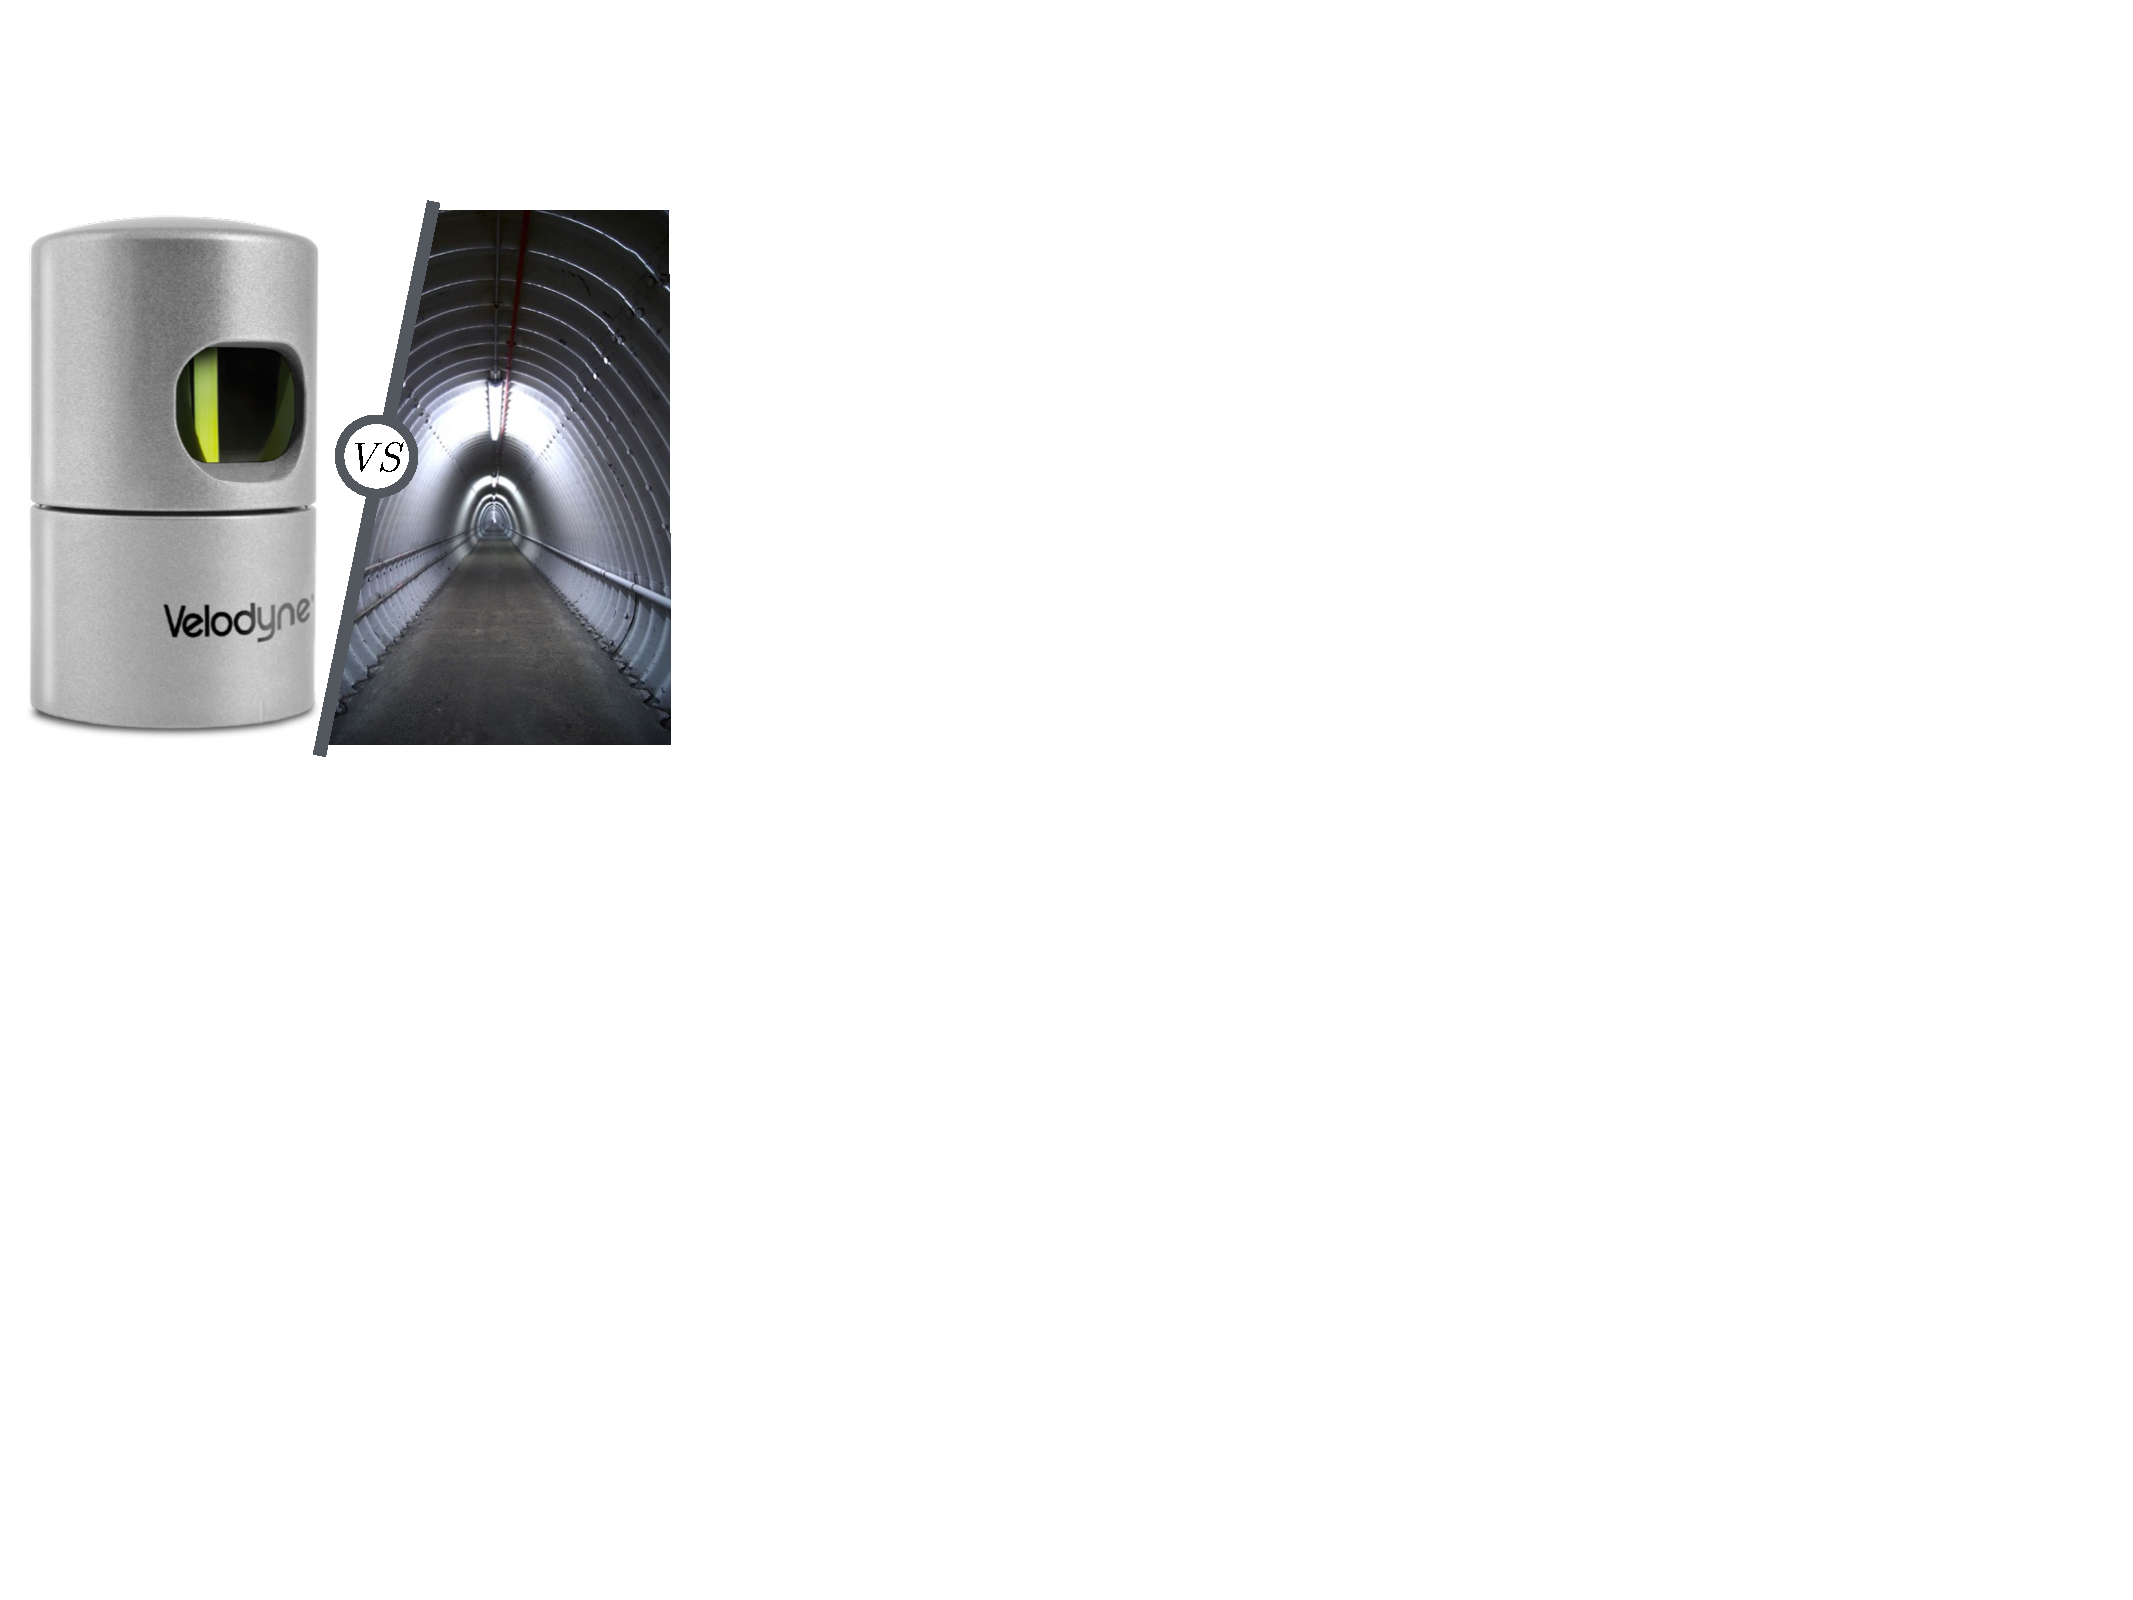
\includegraphics[width=0.35\textwidth]{./figs/overview.pdf}
\caption{
The Velodyne HDL-32E as a maximum range of \SI{100}{\m}, but at those distances distortions starts to appear, specially in long tunnels.
}
\label{fig:overview}
%\vspace{-20pt}
\end{wrapfigure}

Prior work on noise identification \cite{Pomerleau2012} have identified uncertainty models for the Hokuyo URG- 04LX, UTM-30LX, and the Sick LMS-151.
Those models are believed to be pessimistic because the uncertainty related to noise had to be augmented to cope for biases that were not modeled.
One of the hypothesis is that large incidence angles (i.e., the angle between the laser beam and the surface normal vector) produce a constant bias.
This problem is particularly visible when a robot is used to produce a map from a long hallway, tunnel, and even streets seen from faraway.
Better sensor models would have impacts on autonomous mining and autonomous cars.

The goal of this project is to investigate if those biases can be modeled and included in 3D mapping algorithm, such as \cite{Pomerleau2014}.
The final implementation is expected to be implemented in C++ and integrated within \texttt{libpointmatcher} (\url{https://github.com/ethz-asl/libpointmatcher}), a modular library containing multiple algorithms used inside \ac{ICP} and currently used in multiple research projects around the world.
Proof of concept will be demonstrated on existing data sets, starting with the ones collected for \cite{Pomerleau2012}.
New data sets will be recorded using a Velodyne HDL-32e.
Final experiments will be conducted with mobile robot and a Velodyne HDL-32e in underground tunnels connecting buildings on the campus of Laval University (see \autoref{fig:overview}).
If the project goes well, an underground 3D map of the campus could be produced for the first time.

% ---------------------------------------------------------------
\section*{Research Environment}

The project will be hosted by the Northern Robotics Laboratory (norlab) located on the main campus of Laval University.
The university was established in \num{1663}, making it the oldest academic institution in Canada and the first school in North America to offer higher education in French.
It currently enrolls \num{50000} students, from which around \num{9000} are at the postgraduate level.
Norlab is specialized in mobile and autonomous systems working in winter or difficult conditions. 
We aim at investigating new challenges related to navigation algorithms to push the boundary of what is currently possible to achieve with a mobile robot in real-life conditions. 
The current focus of the laboratory is on localization algorithms designed for laser sensors (lidar) and 3D reconstruction of the environment.

% ---------------------------------------------------------------
\printbibliography


\end{document}
